\documentclass[a4paper]{article}
\usepackage[14pt]{extsizes} % для того чтобы задать нестандартный 14-ый размер шрифта
\usepackage[utf8]{inputenc}
\usepackage[english, russian]{babel}
\usepackage{setspace,amsmath}
\usepackage{epigraph} % для эпиграфов и продвинутых цитат
\usepackage{csquotes} % ещё одна штука для цитат
\usepackage[unicode, pdftex]{hyperref} % подключаем hyperref (для ссылок внутри  pdf)
\usepackage{amssymb} % в том числе для красивого знака пустого множества
\usepackage{amsthm} % в т.ч. для оформления доказательств
\usepackage[left=20mm, top=15mm, right=15mm, bottom=15mm, footskip=7mm]{geometry} % настройки полей документа 
\usepackage[active]{srcltx}
\usepackage{indentfirst}
\usepackage{listings}
\usepackage{tocloft}
\usepackage{misccorr} 
\usepackage{graphicx}
\usepackage{caption}
\usepackage[style=numeric,sorting=none]{biblatex}
\DeclareCaptionLabelSeparator{defffis}{ --- }
\captionsetup{justification=centering,labelsep=defffis}
\graphicspath{{images/}}
\DeclareGraphicsExtensions{.jpg}
\renewcommand{\cftsecleader}{\cftdotfill{\cftsubsecdotsep}}
\newcommand{\ran}{{\rm ran}\,}
\newcommand{\diag}{{\rm diag}\,}
% переименовываем  список литературы в "список используемой литературы"
\addto\captionsrussian{\def\refname{Список используемой литературы}}
\addto\captionsrussian{\renewcommand\listfigurename{Список рисунков}}
\newcounter{totreferences}
\pretocmd{\bibitem}{\addtocounter{totreferences}{1}}{}{}
\newtheorem{theorem}{Теорема} % задаём выводимое слово (для теорем)
\newtheorem{definition}{Опредление} % задаём выводимое слово (для определений) 
% объявляем новые команды 
\newcommand{\RNumb}[1]{\uppercase\expandafter{\romannumeral #1\relax}}

\begin{document} % начало документа
\def\figurename{Рисунок}

\makeatletter
\lst@UserCommand\lstlistlistingname{Список листингов кода:}
\makeatother
 
% НАЧАЛО ТИТУЛЬНОГО ЛИСТА
\begin{center}
 \hfill \break
\hfill\break
\hfill\break
\hfill \break
\hfill \break
\hfill \break
\hfill \break
\hfill \break
\hfill \break
\large{\textbf{CORPORATE FOOD CHECKER}}\\
\hfill \break
\hfill \break
\large{\textbf{Система выбора корпоративных обедов на предприятии}}\\
\large{\textbf{Инструкция пользователя}}\\
\hfill \break
\hfill \break
Версия 0.0.1\\
\hfill \break
\hfill \break
\hfill \break
\hfill \break
\hfill \break
\hfill \break
\hfill \break
\hfill \break
\hfill \break
\hfill \break
\hfill \break
\hfill \break
\hfill \break
\begin{center} Санкт-Петербург, 2020 \end{center}
\end{center}
\thispagestyle{empty}
 
% КОНЕЦ ТИТУЛЬНОГО ЛИСТА
 
\newpage 
	\addcontentsline{toc}{section}{Содержание} 
    \tableofcontents % Вывод содержания
\newpage

\section{Назначение и описание программы}

Программа предназначена для автоматизации выбора пользователями готовых обедов на предприятии. Она позволяет выбрать каждому из зарегистрированных пользователей один из нескольких вариантов обеда, доступных на выбранную дату, подтвердить свой выбор и сохранить его. Администратору приложения будет показан отчет на каждую дату, включающий общую статистику по выбранным пользователями обедам.

\section{Интерфейс программы и начало работы}

Интерфейс программы можно условно разделить на две части: простого пользователя и административную панель. При входе на главную страницу будет показано приветственное окно с названием программы и предложение войти под своей учетной записью. Интерфейс адаптивный - можно использовать его как на персональном компьютере с полноценным браузером, так и на мобильном телефоне с современной операционной системой (как Android, так и iOS). На рисунках ~\ref{fig:image1} и ~\ref{fig:image2} показаны внешний вид приложения на разных системах.

\begin{figure}[h]
\center{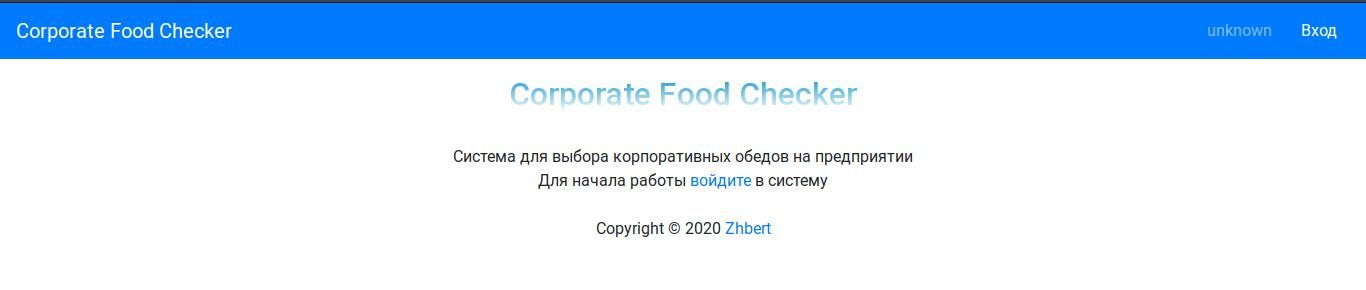
\includegraphics[width=1\linewidth]{001}}
\caption{Главная страница приложения}
\label{fig:image1}
\end{figure}

\begin{figure}[h]
\center{
\includegraphics[scale=0.23]{002}}
\caption{Главная страница приложения на мобильном устройстве}
\label{fig:image2}
\end{figure}

\section{Вход в систему}

Для входа в систему перейдите на страницу входа. Попасть на нее можно либо нажав на кнопку <<\textbf{Вход}>> в верхнем правом углу главного меню, либо пройдя по ссылке <<\textbf{войдите}>> на главной странице.

\begin{figure}[h]
\center{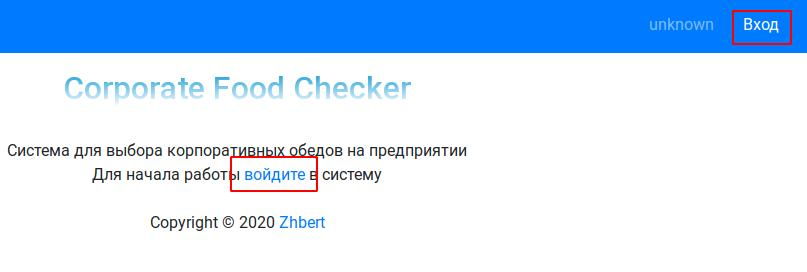
\includegraphics[width=1\linewidth]{003}}
\caption{Кнопка входа и ссылка на страницу входа}
\label{fig:image3}
\end{figure}

В мобильной версии программы кнопка \textbf{<<Вход>>} может быть скрыта в главном меню. Главное меню доступно по нажатию кнопки в верхнем правом углу экрана.

\begin{figure}[h]
\center{
\includegraphics[scale=0.5]{004}}
\caption{Главное меню и кнопка входа в мобильной версии}
\label{fig:image4}
\end{figure}

После нажатия кнопки произойдет переход на страницу входа в систему.

\begin{figure}[h]
\center{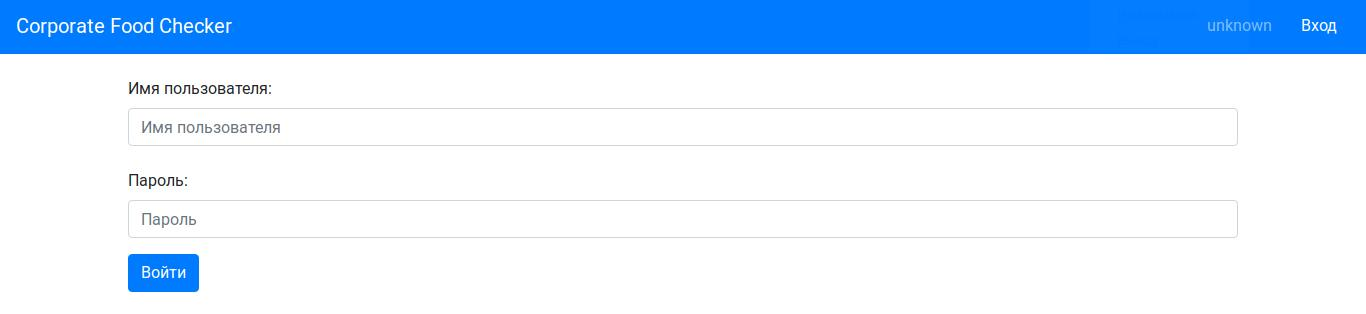
\includegraphics[width=1\linewidth]{005}}
\caption{Страница входа}
\label{fig:image5}
\end{figure}

Для входа введите свои учетные данные\footnote{\textbf{Обратите внимание!} Учетные данные главного администратора приложения выдаются разработчиков при передаче доступа к программе.}.

Введите имя пользователя и пароль в соответствующие поля и нажмите \textbf{<<Вход>>}. Если все прошло правильно, в правом верхнем углу возле кнопки \textbf{<<Вход>>} появится имя пользователя, а в главном меню появятся дополнительные пункты.

\begin{figure}[h]
\center{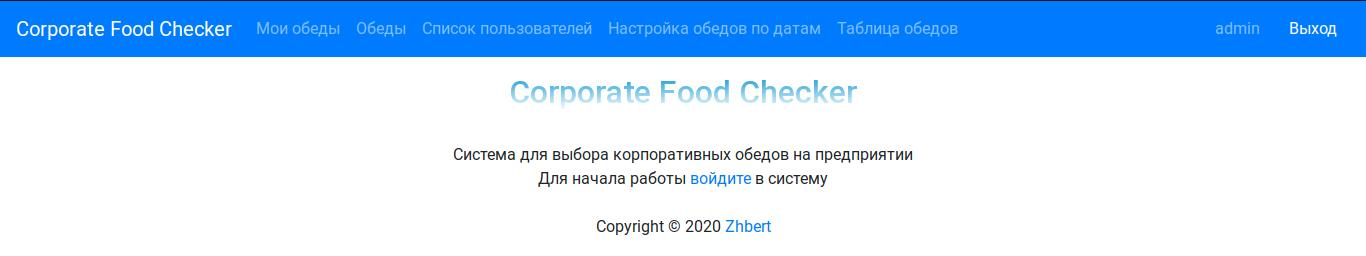
\includegraphics[width=1\linewidth]{006}}
\caption{Главная страница администратора системы}
\label{fig:image6}
\end{figure}

При неправильно введенных данных будет показано соответствующее сообщение об ошибке.

\begin{figure}[h]
\center{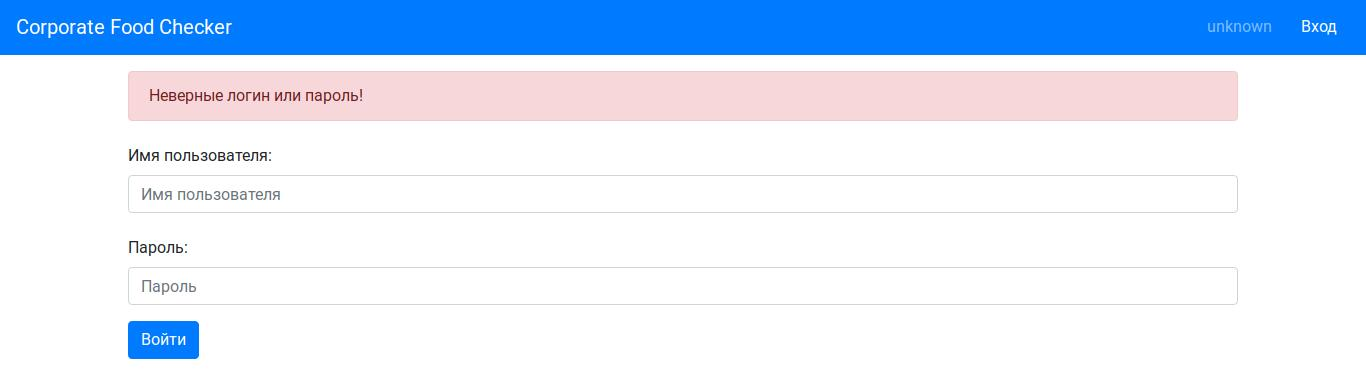
\includegraphics[width=1\linewidth]{007}}
\caption{Сообщение об ошибке входа в систему}
\label{fig:image7}
\end{figure}

\section{Администрирование системы}

\subsection{Алгоритм работы с системой}

Для правильной работы с системой следует выполнять действия в определенном порядке, представленном ниже\footnote{Выполнять действия именно в таком порядке следует только в первый раз. В дальнейшем возможно изменение порядка в зависимости от ситуации}.

\begin{itemize}
\setlength{\itemsep}{-2mm}
	\item \textbf{Создание пользователей} - создание учетных данных пользователей;
	\item \textbf{Создание обедов} - настройка комплексов обедов, доступных для заказа;
	\item \textbf{Настройка обедов по датам} -  присвоение соответствующих обедов конкретным датам;
\end{itemize}

\subsection{Создание пользователей системы}

Для того, чтобы работники предприятия могли выбирать желаемые ими обеды, нужно создать для них учетные записи. Создание производит администратор системы на вкладке \textbf{<<Список пользователей>>}.

\begin{figure}[h]
\center{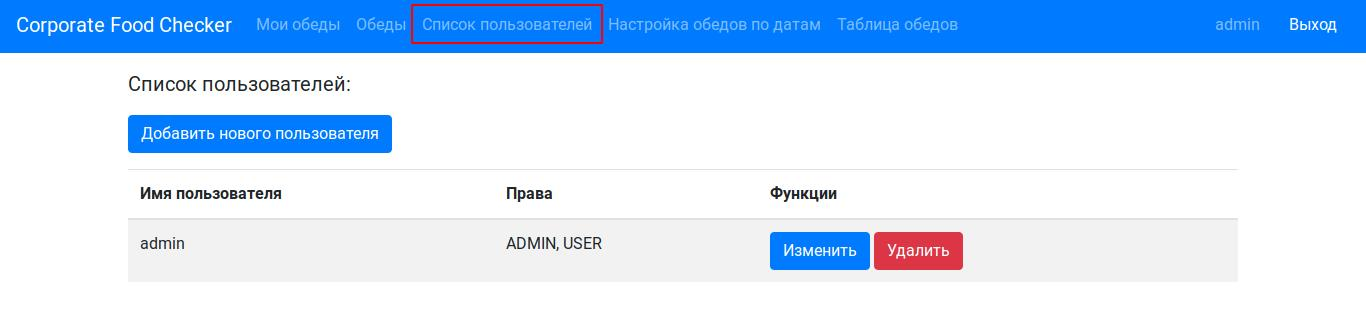
\includegraphics[width=1\linewidth]{008}}
\caption{Сообщение об ошибке входа в систему}
\label{fig:image8}
\end{figure}

Ручное создание учетных записей необходимо для точного соблюдения правильности подсчета: произвольная регистрация предоставит возможность создавать неактивные учетные данные или сделать их задвоение, что нарушит правильность статистики и при большом количестве пользователей будет выдавать достаточно большую погрешность.

На рисунке ~\ref{fig:image8} показана страница пользователей. В таблице представлены все пользователи системы. Таблица имеет три столбца:

\begin{itemize}
\setlength{\itemsep}{-2mm}
	\item \textbf{Имя пользователя} - имя пользователя, необходимое для входа в систему;
	\item \textbf{Права} - права пользователя в системе:
		\subitem \textbf{\textit{ADMIN}} -  администратор системы
		\subitem \textbf{\textit{USER}} - простой пользователь
	\item \textbf{Функции} -  действие, которые можно выполнить с учетной записью:
		\subitem \textbf{\textit{Изменить}} - изменение учетной записи;
		\subitem \textbf{\textit{Удалить}} - удаление учетной записи;
\end{itemize}

\end{document}  % КОНЕЦ ДОКУМЕНТА !